\section{A diamond-blocked Metal engine}\label{sec:gpu}
Section~\ref{sec:ceiling} ends at the memory bus. The fused CPU sweep and the unfused GPU engine of the fork's base
stream every field array from DRAM at least once per time step, and at the 121--127\,GB/s the GPU kernels drew, a fused GPU sweep that
moves 49\,B per cell is bound to about 2\,470--2\,590\,\MC. Temporal blocking moves that bound: a tile of the grid is advanced by $K$
time steps while its fields stay in the GPU's caches, so a field value need not cross the bus at every step. The
fork's engine for this, \code{--engine=metal-diamond}, was written on 2026-11-04 in ten snapshots, cg19 to cg28
(patches 0007--0016, commits 6b23756 to 68c1c82; \code{CHANGELOG.md}). Its tile schedule follows luikore's Metal
engine, openEMS PR~\#228~\cite{luikore228} (GPL; the diamond tile schedule; no code of it is used). The kernels are
the fork's own. They began as a \code{--diamond K} mode of the Swift/Metal prototype of Section~\ref{sec:ceiling},
which matched the CPU engine bit for bit at every $K$ tried (\code{results/diamond\_swift\_2026-11-04.txt}), and were
then moved onto the engine's own arrays and given the extensions that the six models use. The engine is opt-in and
Apple-only: it is built with the base's Metal option (\code{ENABLE\_METAL}), and the default engine stays the
multithreaded CPU engine. The code is \code{FDTD/engine\_metal\_diamond.h} and
\code{FDTD/metal/engine\_metal\_diamond.mm}; against cg18 the ten patches change 19 files, $+1\,717/-1$ lines, of which
the Objective-C++ file has 1\,592 (\code{git diff --stat cb168f7 68c1c82} in the fork). Snapshot cg29 leaves these
files unchanged; its CPU changes were checked against the engine (below). The build of 2026-11-11, cg31 (patches
0028--0039, of which 0029--0038 are the engine's), changes the engine again: this section describes and measures it
as of cg29, and Section~\ref{sec:cg31} has what changed and the rates since.

\subsection{Design}
\paragraph{Fields in shared memory.} \code{Engine\_Metal\_Diamond} is a subclass of the sse-compressed engine, and its
operator is, since cg24, the multithreaded engine's (\code{Operator\_Multithread}). The voltage and current arrays are
the engine's own \code{f4vector} arrays, placed in shared Metal buffers in the unified memory
(\code{ArrayENG::InitView}), so the probes, the dumps and the CPU fallback read and write the memory the kernels use,
without copies. Their order is N-I-J-K, the component outermost, instead of the CPU engines' I-J-K-N, where the three
components of a cell lie side by side and the loads of a SIMD group are 48\,B apart: on Mur boxes of $121^3$ and
$201^3$ cells N-I-J-K ran 7--9\,\% faster (GPU time, three alternating runs each, on a quieter Mac;
\code{results/diamond\_engine\_cg19\_2026-11-04.txt}, section 4). At the first time step the engine copies the
operator's coefficient tables and the extensions' data into Metal buffers and compiles its kernel for the model, with
the stages that the model does not use left out; this GPU setup took 3--33\,ms on the six models
(\code{results/diamond\_engine\_cg24\_cg27\_2026-11-04.txt}, section 5).

\paragraph{Mountains and valleys.} Along x and along y the lines are cut into mountains of width $M$ with valleys of
width $V$ between them; z stays whole in every tile. One threadgroup advances one tile by $K$ time steps, $2K$ half
steps, in place. A mountain $[l,h)$ shrinks as it climbs: at half step $s$ it updates the lines
$[l+\lfloor s/2\rfloor,\,h-\lceil s/2\rceil)$, so every value it reads at its edges is still at the step it needs. A
valley between two mountains, with $l$ the end of the mountain before it and $h$ the start of the one after, grows by
the same rule, $[l-\lceil s/2\rceil,\,h+\lfloor s/2\rfloor)$, and completes what the mountains left. With tiles in x
and in y, a block of $K$ steps takes four dispatches, one per kind of tile: mountain in x and in y, mountain in x and
valley in y, valley in x and mountain in y, valley in both (three since cg31, which sends the two mixed kinds
together; Section~\ref{sec:cg31}). The tiles of one dispatch are independent of each other.
Inside a tile a threadgroup barrier on device memory separates the stages, and the voltage half step from the current
half step. Threadgroup memory is not used: the reuse across the $K$ steps comes from the GPU's caches, and there are
no halo copies. The first mountain starts at line 2 and the last ends at line $n-2$ at the latest, so the two lines at
each domain edge (a Mur face and the line it reads) always lie in one edge valley; a remainder of at least $2K-1$
lines becomes a narrower last mountain, and $M$ must be at least $2K-1$. The host puts whole blocks of $K$ steps into
a command buffer until it holds at least 64 steps (66 at $K=3$) or the call ends, and commits the buffers in order.
An \code{IterateTS} call waits for its last buffer, so the
probes, dumps and end criteria that openEMS evaluates between calls see the fields of that step, on the CPU.

\paragraph{Extensions.} Each extension that touches the fields during a step has a stage in the kernel, run per tile
on the tile's cells, in the CPU engine's order: the Pre stages in reverse extension order, the update, then the Post
and Apply stages in extension order (by priority UPML first, then Mur, lumped RLC and the dispersive materials, the
excitation last; \code{results/diamond\_engine\_cg22\_cg23\_2026-11-04.txt}):
\begin{lstlisting}
E step: [Mur Pre, Lorentz Pre, Debye Pre] -> UPML Pre -> update -> UPML Post -> [Mur Post, Debye Post]
        -> Apply list (Mur faces, lumped RLC, field -= ADE per order) -> voltage excitation
H step: Lorentz Pre -> UPML Pre -> update -> UPML Post -> dispersive current Apply -> current excitation
\end{lstlisting}
The stages in brackets only read the field and run before one barrier.
\begin{itemize}
\item \textbf{Excitation} (cg19): voltage and current sources with their delays and signal periods. At first thread 0
  of every tile scanned all entries at every half step; on a $201^3$ PEC box with 1\,035 voltage entries the rate in
  GPU time was then 1\,914\,\MC, and per-tile lists of the entries in the tile's ranges, kept in entry order, raised it
  to 3\,135 (1\,024 threads per tile, rough; \code{results/diamond\_engine\_cg19\_2026-11-04.txt}, section 5). Since cg25 the entries
  form \emph{runs}: all entries that write one float go to one thread, in the CPU's order, coded in one \code{uint4}
  (the float's index, x and y in 16 bits each, the first and the end entry), so x and y may have at most 65\,535 lines.
\item \textbf{Mur} (cg19): Pre, update, Post and Apply of the face cells in the tile's ranges; the edge valleys keep a
  face and the line it reads in one tile.
\item \textbf{Lumped RLC} (cg20): one state record per element ($I_l$, $V_d[n-1]$, $V_d[n-2]$, $J[n-1]$, $J[n-2]$), in
  the Apply order together with the Mur faces.
\item \textbf{UPML} (cg21): per component and cell an index into a table of distinct coefficient sets, as in the
  CPU's compressed PML tables (cg14). One barrier serves a stage of all boxes, so the boxes must not overlap; openEMS's
  do not (\code{Create\_UPML} leaves out the edges and corners that another box has). Up to cg29 a stage was a loop
  over single floats; since cg31 it takes a z-vector at a time in the x and y slabs and the three components of a
  cell together in a z slab (Section~\ref{sec:cg31}).
\item \textbf{Drude/Lorentz materials and conducting sheets} (cg22, \code{Engine\_Ext\_LorentzMaterial}: voltage and
  current ADEs) and \textbf{Debye materials} (cg23, \code{Engine\_Ext\_DebyeMaterial}), each only as exactly that
  class (\code{typeid}), not as a subclass. Since cg25 the ADE elements of one cell form one run, as the excitation's
  entries do.
\end{itemize}
The extension data sit in three buffers (read-only words, read-only floats, state) with a table of offsets, because
the kernel had used 29 of Metal's 31 buffer slots before the UPML came (cg21). Since cg31 the offsets and counts
are constants of the kernel, which is compiled after the data are packed, and a tiling's per-tile lists have a buffer
of their own (Section~\ref{sec:cg31}).

\paragraph{Coefficients, constants and the tuner.} The packed tables of cg13 hold six \code{f4vector}s per operator
for the voltages and six for the currents, 192\,B per operator. That suits the uniform tutorial meshes, which repeat a
few operators, but the SMA launch's graded mesh (0.871\,M cells, the mesh of the SMA figures in this section) has
64\,410 operators, one for every 3.4 \code{f4vector}s of the grid,
12.4\,MB packed. Split tables (cg27) store
the distinct \code{f4vector}s once, 88\,485 of them in 1.4\,MB for the SMA launch, and per operator a \code{uint4} of
indices for each of the two updates (32\,B), 2.1\,MB (the voltage-voltage and current-current factors first, at most
1\,024 of them for 10-bit indices),
so the caches hold the coefficients of more cells for one more dependent load per cell. They are the default where
the packed coefficients of a $16\times16$ block of (x,~y) columns exceed 32\,KB on average: the SMA launch (275\,KB),
the GCPW line (46\,KB) and the patch tutorial (58\,KB); notch x3 (6\,KB), patch x5 (21\,KB) and the notch tutorial
(9\,KB) stay packed (\code{results/diamond\_engine\_cg24\_cg27\_2026-11-04.txt}, section 4). Since cg26 the grid sizes
are constants of the compiled kernel, so its divisions by them become multiplications. Since cg28 the tiling is
chosen at run time. The engine builds four tilings, $(K,M,V) = (4,8,8)$, the former default, $(4,12,8)$, $(3,8,6)$ and
$(3,6,6)$, each with its own tile buffers, threads per tile and per-tile lists; the extension floats and the state
are shared. While it tunes, the command buffers take the tilings in turn, in half batches of 32 steps (33 at $K=3$)
with at most two in flight, and per tiling the engine keeps the least GPU time per step of four timed buffers; then it runs the
fastest tiling and releases the others (since cg31 seven tilings, timed in two stages: $(4,10,6)$, $(4,9,2)$ and
$(5,12,8)$ are added; Section~\ref{sec:cg31}).
Only full batches and whole calls are timed and take a turn: a first version
that also gave the short last buffer of each call a turn handed one tiling that buffer on every call of notch x3, and
other call lengths could have starved a tiling for a whole run
(\code{results/diamond\_engine\_cg28\_tuner\_2026-11-04.txt}, section 4). Threads per tile follow the tile's work: the
power of two at or below 3/5 of the \code{f4vector}s that a mountain updates per half step ($M\cdot M\cdot n_v$), 256
to 1\,024 (cg21).

\paragraph{Knobs and fallback.} \code{OPENEMS\_DIAMOND\_K} and \code{OPENEMS\_DIAMOND\_TILE} (\code{M,V} or \code{M:V},
default $2K,2K$) fix one tiling, \code{OPENEMS\_DIAMOND\_TUNE=n} sets the timed buffers per tiling (4; \code{0} runs
$K=4$, $8{:}8$ without tuning), \code{OPENEMS\_DIAMOND\_TG} the threads per tile, \code{OPENEMS\_DIAMOND\_BATCH} the
steps per command buffer (64, rounded up to whole $K$-step blocks), \code{OPENEMS\_DIAMOND\_COEF=packed|split} the
coefficient layout, and
\code{OPENEMS\_DIAMOND\_TIMING=1} or \code{2} prints the GPU time, per phase with \code{2} (which also fixes one
tiling). cg31 adds eight switches for its changes (Section~\ref{sec:cg31}; all in \code{BUILD.md}, section 7).
Whatever the engine does not
cover runs on the CPU, on the same memory, with a message: an extension without a GPU stage (named in the message;
TFSF, the steady-state detection, any subclass of the dispersive extensions), overlapping UPML boxes, more than
65\,535 lines in x or y, $2^{32}$ or more floats per field, no Metal device or a failed allocation; more than 32 Mur
faces or UPML boxes, or more than 65\,535 lumped-RLC or dispersive extensions, fall back without a message. The
fallback is the sse-compressed engine's generic loops on one thread; at cg19 the six models all ran it, and their speeds there
mean nothing (\code{results/diamond\_engine\_cg19\_2026-11-04.txt}, section 2). Cylindrical meshes run openEMS's
cylinder engine whatever the option says. Table~\ref{tab:gpucov} lists what each snapshot put on the GPU.

\begin{table}[htbp]\centering\small
\resizebox{\textwidth}{!}{%
\begin{tabular}{@{}lll>{\raggedright\arraybackslash}p{6.3cm}p{3.6cm}r@{}}
\toprule
snapshot & patch & commit & added on the GPU, or changed & benchmark models on the GPU & \code{diamond\_check} \\
\midrule
cg19 & 0007 & 6b23756 & cell updates; voltage and current excitation with delays and periods; Mur & none & 18 \\
cg20 & 0008 & 7ac3438 & lumped RLC elements & patch tutorial, patch x5 & 24 \\
cg21 & 0009 & 2c79751 & UPML; extension data in three buffers; threads per tile from the tile size &
  + notch tutorial, notch x3, SMA launch & 36 \\
cg22 & 0010 & 5ea5ffd & Drude/Lorentz materials and conducting sheets & + GCPW line: all six & 48 \\
cg23 & 0011 & 0242c5f & Debye materials & all six & 54 \\
cg24 & 0012 & 8dd56e5 & operator setup on all cores (\code{Operator\_Multithread}); \code{OPENEMS\_DIAMOND\_TIMING} &
  all six & 54 \\
cg25 & 0013 & 3db2791 & excitation and dispersive elements as runs; per-tile offsets read once & all six & 54 \\
cg26 & 0014 & ca7c334 & grid sizes as constants of the kernel; Mur and UPML records passed by value & all six & 54 \\
cg27 & 0015 & 282707b & split coefficient tables for graded meshes & all six & 54 + 54 \\
cg28 & 0016 & 68c1c82 & tiling chosen at run time & all six & 72 \\
\bottomrule
\end{tabular}}
\caption{What runs on the Metal diamond engine, per snapshot (all of 2026-11-04). A model runs on the GPU when each
of its extensions has a GPU stage; the others run the CPU loops (at cg19 all six: each has PML, lumped ports or
conducting sheets). \code{diamond\_check}: comparisons of every exported field value of the box models with the
multithreaded engine run with \code{OPENEMS\_FTZ=1}, all identical (\code{results/diamond\_engine\_cg19\_2026-11-04.txt}
to \code{results/diamond\_engine\_cg28\_tuner\_2026-11-04.txt}; the logs of cg21--cg23 are
\code{results/diamond\_check\_cg2N\_2026-11-04.txt}); on cg27 54 more with the split tables forced. cg24's 54 of 54
is recorded only in its commit message (patch 0012), not in \code{results/}; the 180 runs of the cg24--cg27 session,
all equal to the first run of cg24, the CPU engine with \code{OPENEMS\_FTZ=1} among them, show its identity on the six
models as well. cg29 changes only CPU code; its \code{diamond\_check} is 72 of 72
too (\code{results/cpu\_items\_cg29\_2026-11-05.txt}, section 3). Never on the GPU: TFSF, steady-state detection and
subclasses of the dispersive extensions (CPU loops), cylindrical meshes (openEMS's cylinder engine).}
\label{tab:gpucov}
\end{table}

\subsection{Bit identity}
The engine is held to the fork's rule (Section~\ref{sec:policy}) against the CPU engine whose arithmetic it repeats.
Every value gets the CPU engines' operations in the same order. Each component of the cell update is the rounded
product and the one fused multiply-add that Apple clang makes of the CPU expression on arm64:
\begin{lstlisting}
v = volt[...];  v = v * vv;  v = fma(vi, ((c2 - c2ym) - c1) + c1zm, v);  volt[...] = v;   // the currents alike
\end{lstlisting}
\code{fma()} is written where clang fuses, \code{\#pragma METAL fp contract(off)} holds everywhere else, and Metal's
safe math mode is set (fast math off). The extension stages keep the CPU engine's order and their own operation order,
and an excitation run applies the entries of one float in entry order. The tiles, the tiling the tuner picks and the
batch size change only the order in which independent values are computed. One difference remains: Apple's GPU
flushes subnormal floats to zero, while the CPU cores keep them unless \code{OPENEMS\_FTZ=1} sets \code{FPCR.FZ}
(Section~\ref{sec:ceiling}). The reference is therefore the multithreaded engine run with \code{OPENEMS\_FTZ=1}:
\begin{itemize}
\item \code{scripts/checks/diamond\_check.sh} compares every exported field value of box models after the run: PEC
  and Mur boxes; mixed faces with a delayed voltage excitation, a soft current excitation and an excitation on a Mur
  plane; 16 lumped RLC elements; PML on all six faces and PML mixed with Mur; two conducting sheets; Drude/Lorentz and
  Debye blocks. Each runs at $K=1$, 2, 3, 4 and 8 and with an odd tile (7,0), 96 threads and batches of 3 steps, and
  since cg28 also with the tuner changing tilings during the run. Every comparison was identical, 18 at cg19, 24 at
  cg20, 36 at cg21, 48 at cg22, 54 at cg23 to cg27 (cg24's in its commit message), 72 at cg28 and cg29
  (Table~\ref{tab:gpucov}), and 72 at every snapshot of cg31 (Section~\ref{sec:cg31}).
\item The six benchmark models: port probes and $S$-parameters identical to the multithreaded engine with
  \code{OPENEMS\_FTZ=1} on every model that ran on the GPU, two at cg20, five at cg21 and all six from cg22 on
  (\code{results/*\_cg2Ngpu.txt}; for cg29 \code{results/*\_cg29gpu.txt}). The 180 runs of the cg24--cg27 session were
  all identical to the first run of cg24, and the 190 runs of the two cg28 sessions to the first run of cg27
  (\code{results/diamond\_engine\_cg24\_cg27\_2026-11-04.txt}, section 3;
  \code{results/diamond\_engine\_cg28\_tuner\_2026-11-04.txt}, section 1). The Metal runs of cg31 give the probes of
  cg29's (\code{results/metal\_engine\_cg31\_2026-11-11.txt}).
\item The nf2ff time-domain dumps of the patch tutorial (984 datasets) and of patch x5 (120) are identical when both
  runs set \code{OPENEMS\_FTZ=1}. With the switch in the CPU run only, 27 of the tutorial's 984 differed while the
  fields were identical, because openEMS computes the dumps on the creating thread, which the switch also flushes
  (\code{results/diamond\_engine\_cg20\_2026-11-04.txt}).
\item The closed-form validation suite (\code{bench/validation/}) passes 15 of 15 on the engine at cg23 and at cg27
  (and at cg30l, the snapshot of patches 0001--0038 on the way to cg31, Section~\ref{sec:cg31}).
  The Debye, Drude and Lorentz slabs, the rectangular cavity, the WR-90 guide with PML and the microstrip line ran on
  the GPU without a fallback, and the three dispersive slabs equal the basic engine (difference 0); the cylindrical
  cavity runs openEMS's cylinder engine (\code{results/validation\_cg23\_metal.md},
  \code{results/validation\_cg27\_metal.md}).
\end{itemize}
The base's GPU engine (\code{--engine=gpu}, the pre-merge branch at 7bb294f), compared the same way, is identical to
the multithreaded engine with \code{OPENEMS\_FTZ=1} on all six models too (\code{results/*\_cg22gpu.txt}); upstream
master's merged engine was not compared with a run that flushes subnormals (Section~\ref{sec:policy}). Against stock
v0.37.0, which keeps subnormals, the diamond engine's differences are those of the flush. They are measured, not
acceptance criteria: $1.7\times10^{-7}$ to $9.4\times10^{-7}$ relative in the port probes, at most
$2.3\times10^{-4}$\,dB in $S_{11}$ (notch tutorial; at most $2.3\times10^{-5}$\,dB on the other models) and at most
$9.4\times10^{-5}$\,dB in $S_{21}$ (\code{results/*\_cg22.txt}; the GPU results have not changed since). End to end
through the toolkit (cg23, CPU runs without the flush) the runs stop at the same steps; $S_{11}$ of the SMA launch
differs by at most $7.3\times10^{-3}$\,dB ($-22.69$\,dB at 1\,GHz in all four runs), $S_{21}$ by at most
$2.0\times10^{-4}$\,dB, and on the GCPW line $S_{21}$ by at most $3.9\times10^{-6}$\,dB
(\code{results/rfsim\_e2e\_gpu\_2026-11-04.txt}).

\subsection{Speed}
The Mac was shared during this work. The cg19 to cg23 runs were made on a loaded Mac (load averages of 2 to 8 where
the files give them), and in the cg24--cg27 sessions other jobs took 0.5--7.7 cores and up to 31\,\% of the GPU; the
files call single runs rough, and the comparisons that count are paired. Of the comparisons of cg19 to cg28 only cg28's ran on a quiet Mac; the cg29 size sweep below waited for one before every run. Ratios are paired and interleaved
(Section~\ref{sec:method}): the median of the per-round ratios, with their range.

\paragraph{When the GPU wins.} On Mur boxes at cg19 (rough, load average 2--7) the engine at $K=4$ ran 2\,447\,\MC\ on
$121^3$ cells and 2\,775 on $201^3$, against 1\,795 and 1\,579 for the multithreaded engine of the same build (the CPU
code of cg18) at 8 threads and 1\,472 and 1\,446 for the base's GPU engine. On $61^3$ cells (0.23\,M) the CPU at 4
threads was faster, 2\,281 against 2\,099 (\code{results/diamond\_engine\_cg19\_2026-11-04.txt}, section 3): that model
did not fill the GPU, and whether a small model loses on the GPU also depends on the CPU's rate there (on cg29 the
GPU led on the GCPW line at 0.11\,M cells, below). The six models' rates on this engine at cg29, next to stock and
cg29 on the CPU, are in
Table~\ref{tab:current}, which runs the SMA launch on its 1.071\,M-cell mesh; their rates at cg31 are in
Table~\ref{tab:cg31}.

\paragraph{Where the GPU overtakes the CPU.} There is no single size at which the GPU becomes the faster engine; it
depends on the model. Three models were run at several mesh scales on cg29 (Figure~\ref{fig:crossover};
\code{results/gpu\_crossover\_cg29\_2026-11-05.txt}): the patch antenna of the patch tutorial from 0.10 to 7.9\,M cells
(scale 1 is the patch tutorial, scale 5 patch x5), the notch filter of the notch tutorial from 0.27 to 5.2\,M (scale 3
is notch x3) and the GCPW line from 0.11 to 5.1\,M, 25 points, each in 4 paired, interleaved rounds of the
multithreaded engine at 8 and 4 threads and the GPU engine with and without its timing (others' CPU 0.5--1.3 cores
and GPU 1--5\,\% in the median of a point; every run waited, for up to 30 minutes, until the others used at most 1.5 cores and
10\,\% of the GPU, and was repeated up to three times when they used more; a round still loaded after that was left
out where two clean rounds remained, so 9 points rest on 3 rounds and 2 on 2). The multithreaded engine was fastest at 8 threads at every point. The GPU was ahead in every
round from 1.7\,M cells on the notch filter, from 2.4\,M on the GCPW line and from 2.9\,M on the patch antenna, by
1.10--1.52$\times$ from there and by 1.25--1.52$\times$ from 3.1\,M cells on; the medians cross for the last time at about 0.66, 1.45
and 1.91\,M cells. Below that the two engines were within 0.89--1.23$\times$ of each other and the side depended on
the model: the GPU led on the GCPW line at 0.11--0.42\,M cells (1.03--1.23$\times$), trailed on the notch filter
(0.89$\times$ at 0.27\,M, 0.97$\times$ at 0.50\,M) and changed sides from size to size on the patch antenna
(0.94--1.11$\times$ up to 1.85\,M). On grids this small the session counts as well: the patch tutorial, 1.107$\times$
[1.09--1.17] in the sweep, ran 0.95--0.97$\times$ in two later runs of the same 36\,500 steps on a quieter Mac and
0.91--0.93$\times$ at the bench's 10\,500 steps, with the CPU 8\,\% faster than in the sweep and the GPU 6\,\% slower
(section 5 of the file). Every CPU run gave the CPU reference's probes; the GPU's differed from them by at most
$1.7\times10^{-6}$ relative (no FTZ in either), except at one point where the wave had not yet reached a port and the CPU's values there were
subnormal, which the GPU flushes to zero.

Three things narrow the GPU's lead on smaller grids, or reverse it. \emph{It waits for the CPU.} Between \code{IterateTS}
calls the CPU records the probes and evaluates the dumps while the GPU idles, and starting and finishing a call's
command buffers leaves it idle too: 0.3--0.5\,ms per call on the smallest grids. On the patch tutorial a call ends
every 31 steps, at the nf2ff dumps, and holds 1.3\,ms of GPU work, so the GPU was busy 73--82\,\% of the time-stepping
loop; at 0.62\,M cells 94\,\%, from 4.2\,M 98--99\,\%. On the patch antenna, up to 0.62\,M cells, its rate over busy time alone,
2\,413--2\,898\,\MC, was above the CPU's at every point (1\,766--2\,825): on those grids the waiting decides. The notch
filter and the GCPW line end a call every 81 to 750 steps and kept the GPU busy 97--99\,\% at every size, the notch
tutorial included. \emph{Its own rate is lower on small grids:} over busy time 1\,959\,\MC\ on the notch filter at
0.27\,M cells against 3\,239 at 5.2\,M, and 1\,799--1\,956 on the GCPW line at 0.11--0.16\,M against 3\,053 at
5.1\,M. A dispatch there has few tiles for the 10 GPU cores (75--96 tiles of 256 threads on the notch filter at 0.27\,M,
18--30 on the GCPW line at 0.11\,M) and short columns (4 $z$-vectors), and the edge work makes up
more of the cells: the 8-cell PML and the Mur faces on the notch filter, the conducting sheets and the Mur faces on
the GCPW line. These causes were not separated; the patch tutorial, with 16--25 tiles and 12 $z$-vectors, ran
2\,420--2\,510\,\MC\ over busy time. \emph{The CPU is at its best in the middle of the range:} 1\,573--2\,208\,\MC\ at
0.10--0.27\,M cells, 2\,570--3\,003 at 0.62--1.85\,M, above the 2\,273\,\MC\ the cores reach from DRAM
(Section~\ref{sec:ceiling}), presumably because the caches then hold part of the traffic (not measured), and
1\,919--2\,263 at 4.2--7.9\,M, while the GPU ran 2\,818--3\,220 there. The GPU's lead is largest where the CPU is held
to the bus. Refined to 3.2 and 5.1\,M cells, the GCPW line ran 2\,933 and 3\,028\,\MC\ on the GPU, between patch x5
(2\,908) and notch x3 (3\,220): the board's lower rate at its own size, 2\,099 at 0.24\,M cells, comes mostly from
that size and what comes with it (fewer tiles, shorter columns, a larger share of sheet and Mur cells; not separated).

\begin{figure}[htbp]\centering
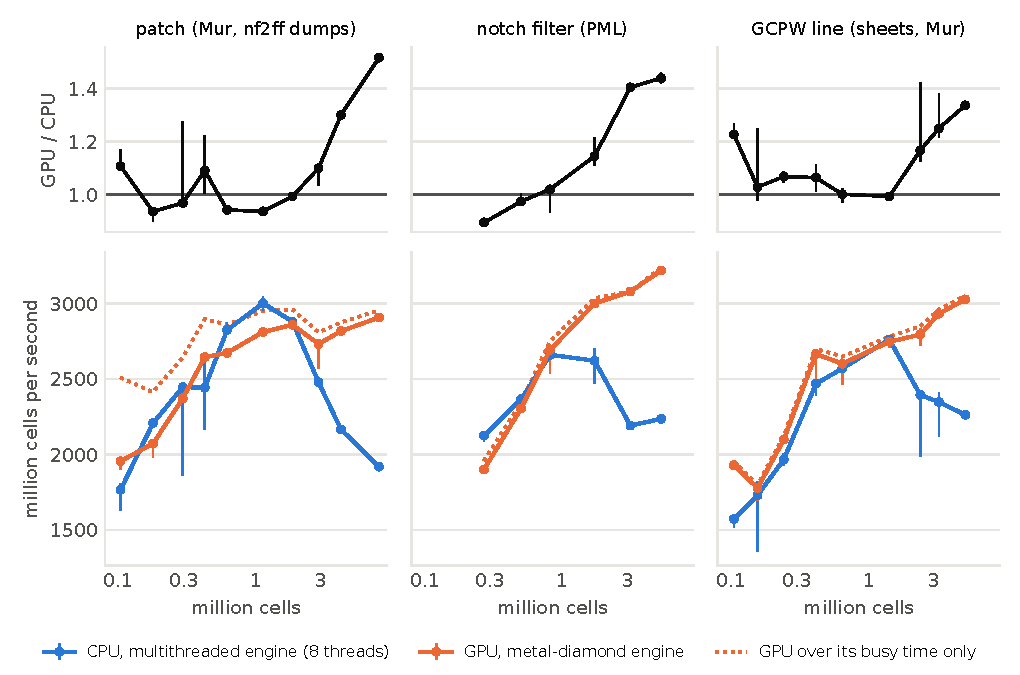
\includegraphics[width=\textwidth]{fig_crossover}
\caption{GPU against CPU by grid size on cg29 (\code{results/gpu\_crossover\_cg29\_2026-11-05.txt}). Top: the GPU
engine's speed over the multithreaded engine's at 8 threads, median of the paired rounds used and their range (4
rounds per point; 9 points rest on 3 and 2 on 2, see the text). Bottom: the medians in \MC\ with the range over the
same rounds; the dotted line is the GPU's rate over its busy time alone
(\code{OPENEMS\_DIAMOND\_TIMING=1}), so the gap down to the GPU's own line is time it waited for the CPU. The patch
and notch meshes are refined by the bench's scale factor (the tutorials at scale 1, patch x5 and notch x3 at scales 5
and 3); the GCPW line's scale multiplies its cell size (scale 1 is the 0.242\,M-cell line of the tables, scales 2 to
0.3 give 0.105 to 5.1\,M cells); logarithmic cell axis.}\label{fig:crossover}
\end{figure}

\paragraph{Tiles and $K$.} No one tiling is best for every model. In a sweep on cg23 (the faster of two runs, others'
CPU 0.4--2 cores, GPU up to 15\,\%) the default $K=4$ with 8:8 tiles was best or within 8\,\% on the four models built
from the tutorials and 8--9\,\% below the best setting on the two boards. In paired runs against the default the
SMA launch gained 1.132$\times$ [1.107--1.144] with $K=2$ and 6:4 tiles (cg24) and the GCPW line 1.114--1.117$\times$
per round with $K=4$ and 12:8 tiles (cg23; \code{results/diamond\_engine\_cg24\_cg27\_2026-11-04.txt}, section 8). The
run-time tuner of cg28 (above) chooses among four tilings. In the cg23 sweep four of the six models ran best with one
of them, and the SMA launch and the patch tutorial with a
$K=2$ tiling, 0.3 and 1.2\,\% faster than the best of the four; in a $K$ sweep on cg27 (the faster of two runs, not
paired; \code{results/fused\_sweep\_k1\_2026-11-04.txt}, part B) the default $K=4$ with 8:8 tiles beat $K=2$ with 4:4 tiles
and every $K=1$ tiling on all six models. $K=2$ with 6:4 tiles, the SMA launch's best in the paired runs of cg24
(against 1.065$\times$ for $K=3$ with 8:6 tiles), is not among the four, nor among the seven of cg31
(Section~\ref{sec:cg31}), and was not timed after cg24 up to cg29; the record of the sweep of thirteen tilings of
2026-11-11 does not list its tilings (\code{results/diamond\_engine\_cg28\_tuner\_2026-11-04.txt}, header;
\code{results/metal\_engine\_cg31\_2026-11-11.txt}).
The earlier fixed 1\,024 threads per tile cost 44\,\% on the notch tutorial and 21\,\% on the SMA launch against the
rule above (loaded Mac; \code{results/diamond\_engine\_cg21\_2026-11-04.txt}, section 4).

\paragraph{From cg24 to cg27.} The operator setup of cg24 runs on all cores: before it, the diamond engine set up
notch x3 in 5.55\,s and patch x5 in 6.48\,s, now in 2.74 and 1.69\,s, against 2.61 and 1.60 for the multithreaded
engine (loaded Mac; \code{results/diamond\_engine\_cg24\_cg27\_2026-11-04.txt}, section 5). A diagnostic build that
leaves parts of the work out (results not identical by design; 3 rounds) showed where the boards' time went: the SMA
launch ran 1.343$\times$ faster without the UPML, 1.257$\times$ with every cell on one operator and 1.167$\times$ without
the excitation, the GCPW line 1.514$\times$ without the sheets and 1.283$\times$ without Mur (section 7). The excitation
and the sheets became runs (cg25), the coefficients split tables (cg27); in one build, split against packed gave
1.053$\times$ [1.03--1.07] on the SMA launch and 1.031$\times$ [1.03--1.04] on the GCPW line (8 rounds, others 4--5
cores). Paired in one session against cg24 (5 rounds; others 4--5.6 cores, load average 11.7--25.2), cg27 ran the SMA
launch 1.265$\times$ [1.22--1.28] faster (median 1\,184 to 1\,482\,\MC) and the GCPW line 1.303$\times$ [1.29--1.37]
(1\,361 to 1\,773). The notch tutorial, notch x3 and patch x5 stayed within noise (0.983--1.012$\times$); the patch
tutorial's 1.251$\times$ [0.93--1.47] rests on 343 short calls under that load and is noise (section 3). Folding the
UPML stages into the cell update gave nothing (paired against cg24, 4 rounds: SMA launch 1.023$\times$
[0.934--1.106], notch tutorial 0.948$\times$, notch x3 0.988$\times$) and was removed (section 1).

\paragraph{Where the GPU waits.} With \code{OPENEMS\_DIAMOND\_TIMING} the engine reports its GPU time. On cg24 the GPU
was busy 96--99\,\% of the time-stepping loop on the two boards and notch x3 and 91\,\% on patch x5, but 78\,\% on the
patch tutorial and 76\,\% on the notch tutorial, whose \code{IterateTS} calls are short (31 steps between the patch
tutorial's nf2ff dumps, 81 on the notch tutorial) and leave the GPU idle while the CPU works between them. On cg29, in
the size sweep above, the patch tutorial kept the GPU busy 79--82\,\% of the loop (73--79\,\% in later runs), but the
notch tutorial 97\,\% with the same 81-step calls: its cg24 figure, from a loaded Mac, was not reproduced. Timed per
phase, notch x3 spent 12/17/18/53\,\% of the GPU time in the four kinds of tile, against a work split of
10/18/18/54\,\% at $M=V=8$, $K=4$: per cell update the four cost the same
(\code{results/diamond\_engine\_cg24\_cg27\_2026-11-04.txt}, section 6).

\paragraph{The run-time tuner (cg28).} Table~\ref{tab:gpuspeed}(a) gives the paired comparison with cg27 on a quiet
Mac: 1.094$\times$ on the SMA launch, 1.114$\times$ on the GCPW line, 1.061$\times$ on notch x3 and 1.064$\times$ on
the patch tutorial. On the notch tutorial and patch x5 the default is the best tiling; there the tuning, 575 and 623
steps with the other tilings in turn, costs 0.4--0.5\,\% of these short runs, and less in real runs of 34\,000 to
190\,000 steps. The choices were those of the best fixed tiling in the paired sweeps and the same in every repeat
(\code{results/diamond\_engine\_cg28\_tuner\_2026-11-04.txt}, sections 2 and 3).

\paragraph{Fused but not blocked ($K=1$).} At $K=1$ a threadgroup updates the voltages and then the currents of its
tile in one pass, and the four kinds of tile complete the tile edges, so each field value is read and written once
per step: the 49\,B per cell of the CPU's fused sweep, the case that Section~\ref{sec:ceiling} bounds at
2\,470--2\,590\,\MC. Measured on cg27 (Table~\ref{tab:gpuspeed}(b); paired, 4 rounds, others' CPU 2.5--4 cores, GPU
3--5\,\%), it ran notch x3 at 1\,716--1\,733\,\MC\ and patch x5 at 1\,530--1\,844 over three tile sizes, 0.54--0.65
times $K=4$. At each model's best tile that is 1.25--1.30 times the base's unfused GPU engine (ratio of the medians),
67--75\,\% of the bound, and 85--90\,GB/s at 49\,B per cell, where the streaming kernels drew 121--127\,GB/s; against
the CPU best of cg18 on a quiet Mac, a comparison across sessions, it is 0.85 (notch x3) and 1.07 times (patch x5)
(\code{results/fused\_sweep\_k1\_2026-11-04.txt}). The per-step structure (four dispatches, the tile edges, a
threadgroup barrier between the two half steps) costs more than the bytes it saves; the bound is a traffic bound only.
Blocking over time steps does what fusing alone does not: $K=2$ (2\,123 and 2\,408\,\MC) is still below the bound,
$K=4$ (2\,986 and 2\,817) above its upper end on both models. A one-dispatch fused kernel was not built: tiles that
compute their own edges would overwrite values their neighbours still read in the same dispatch, so it needs a second
copy of both fields, and every extension would have to follow.

\paragraph{End to end.} Through the author's toolkit (cg23; one run each, another session's job on one core, load
average 2.6--8.0) the engine cut the toolkit's default runs (probe end $-60$\,dB, hold 0.5) from 7.43 to 5.95\,s on
the GCPW line (1.25$\times$) and from 43.71 to 34.23\,s on the SMA launch at 0.871\,M cells (1.28$\times$), and the
full runs to \code{max\_time} by 1.15$\times$ and 1.26$\times$ (\code{FDTD.Run} wall time), against the multithreaded
engine of the same build with its automatic thread count (\code{results/rfsim\_e2e\_gpu\_2026-11-04.txt}). On cg27, under a heavier load, the GPU
runs gave the same port data (\code{results/diamond\_engine\_cg24\_cg27\_2026-11-04.txt}, section 9). The end-to-end
runs of cg29 are in Section~\ref{sec:results}.

\begin{table}[htbp]\centering\small
\textbf{(a)} cg28 (tiling chosen at run time) against cg27, paired, 5 rounds; quiet Mac (others' CPU 0.5--1.3 cores,
GPU 2--4\,\%)\\[3pt]
\resizebox{\textwidth}{!}{%
\begin{tabular}{@{}lrrllll@{}}
\toprule
model (cells, steps) & cg27 & cg28 & cg28 / cg27 & \code{TUNE=0} / cg27 & tiling chosen & tuning steps \\
\midrule
SMA launch (0.871\,M, 6000)      & 1671 & 1828 & 1.094 [1.092--1.097] & 1.001 [0.999--1.003] & $K=3$, 8:6  & 584 \\
GCPW line (0.242\,M, 15000)      & 1896 & 2113 & 1.114 [1.068--1.117] & 0.999 [0.963--1.003] & $K=4$, 12:8 & 588 \\
notch x3 (5.247\,M, 3000)        & 3039 & 3226 & 1.061 [1.061--1.064] & 0.998 [0.996--1.000] & $K=4$, 12:8 & 614 \\
patch tutorial (0.104\,M, 10500) & 1640 & 1764 & 1.064 [1.010--1.152] & 1.000 [0.942--1.042] & $K=3$, 6:6  & 532 \\
notch tutorial (0.270\,M, 16000) & 1908 & 1902 & 0.996 [0.994--1.001] & 0.998 [0.994--1.002] & $K=4$, 8:8  & 575 \\
patch x5 (7.863\,M, 2400)        & 2930 & 2917 & 0.995 [0.994--0.997] & 1.003 [1.002--1.005] & $K=4$, 8:8  & 623 \\
\bottomrule
\end{tabular}}

\vspace{8pt}
\textbf{(b)} The fused, unblocked sweep ($K=1$) on cg27, paired, 4 rounds (others' CPU 2.5--4 cores, GPU 3--5\,\%);
\MC\ (ratio to $K=4$)\\[3pt]
\resizebox{\textwidth}{!}{%
\begin{tabular}{@{}lrrrrrr@{}}
\toprule
model (cells) & base GPU engine (unfused) & $K=1$, 8:8 & $K=1$, 16:8 & $K=1$, 32:16 & $K=2$, 4:4 & $K=4$, 8:8 \\
\midrule
notch x3 (5.247\,M) & 1330 (0.446) & 1716 (0.573) & 1729 (0.579) & 1733 (0.579) & 2123 (0.710) & 2986 \\
patch x5 (7.863\,M) & 1469 (0.515) & 1799 (0.637) & 1844 (0.649) & 1530 (0.541) & 2408 (0.852) & 2817 \\
\bottomrule
\end{tabular}}
\caption{Speed of the Metal diamond engine, \MC\ (medians of the rounds; a ratio is the median of the per-round
ratios, with its range). Tiles are $M$:$V$. (a) \code{results/diamond\_engine\_cg28\_tuner\_2026-11-04.txt}, section 3;
the tiling chosen and the steps the tuning took come from one separate run per model (section 2; others about 0.5--1
core), and the choice was the same in every repeat. \code{TUNE=0} is cg28 with \code{OPENEMS\_DIAMOND\_TUNE=0}, the
fixed $K=4$, 8:8 of cg27. (b) \code{results/fused\_sweep\_k1\_2026-11-04.txt}, part A. The base GPU engine is
\code{--engine=gpu} of the fork's base (7bb294f), not upstream master's merged engine. The traffic bound of a fused
sweep at 49\,B per cell is about 2\,470--2\,590\,\MC\ (Section~\ref{sec:ceiling}). Every run of both sessions equals
its session's first run, and so the multithreaded engine with \code{OPENEMS\_FTZ=1}.}
\label{tab:gpuspeed}
\end{table}

\subsection{Limits and open questions}
\begin{itemize}
\item \textbf{One machine.} Everything here ran on the base M5 with its 10 GPU cores, whose bus the CPU shares. The M5
  Pro (307\,GB/s~\cite{macmini}) was measured later, with cg31, as a set of its own (Section~\ref{sec:m5pro}); the M5
  Max and the M5 Ultra (1.2\,TB/s~\cite{studiom5}) were not measured; for
  luikore's engine, 1.3--4.2$\times$ its own unfused path is reported on an M4 Pro and an M5 Max~\cite{luikore228}.
\item \textbf{No head-to-head with luikore's engine on the six models.} On this M5 its diamond path refused all six
  models (Mur faces; on the GCPW line also the conducting sheets) and ran only variants with every Mur face replaced
  by PEC, on which this engine was not run (\code{results/others\_2026-11-04/}, Section~\ref{sec:ceiling}). Since
  2026-11-11 there is one on luikore's own benchmark model, a uniform grid with PEC walls: cg31's engine ran 3\,981
  and 3\,309\,\MC\ at 3.0 and 17.0\,M cells, luikore's 3\,952 and 2\,829 (Section~\ref{sec:threebuilds},
  Table~\ref{tab:threebuilds}). Its diamond path still refuses the six models.
\item \textbf{No bytes per cell.} The traffic model of Section~\ref{sec:fused} gives the bytes of a sweep that streams
  every array once or twice per step. With $K$ steps per tile the traffic depends on what the caches keep, and it was
  not measured with hardware counters, so this engine has no bytes-per-cell figure and no bar in
  Figure~\ref{fig:bandwidth}. Its rates above the bound show only that it moves less than 49\,B per cell update.
  Section~\ref{sec:cg31} adds a count from the tile schedule, 20--29\,B of field per cell and step for a tile that
  stays cached through its block; it is a count, not a measurement.
\item \textbf{GPU memory} was not measured: the shared field buffers, the four tilings' buffers while tuning (seven
  tilings since cg31), the extension buffers. Only the coefficient tables are known (above).
\item \textbf{Graded meshes and extension work.} The boards run below the large uniform models, for their UPML, sheet
  and excitation work and their many distinct operators (the ablation above), and for their size: refined to 3.2 and
  5.1\,M cells, the GCPW line ran between patch x5 and notch x3 (Figure~\ref{fig:crossover}). The SMA launch,
  1\,829\,\MC\ at 1.07\,M cells in Table~\ref{tab:current} against 2\,747--2\,812 for the GCPW line and the patch
  antenna at 1.1--1.4\,M cells in the size sweep (another session), was not scaled. The tuner picks among four tilings
  only. Since cg31 (Section~\ref{sec:cg31}) a block takes three dispatches, the UPML and the dispersive stages take a
  z-vector or the three components of a cell at a time, Mur faces of one axis share a barrier and the tuner has seven
  tilings: the GCPW line and the SMA launch (0.871\,M cells) gained 1.09$\times$ and 1.14$\times$
  (Table~\ref{tab:cg31}). The extensions still cost, and the cost is tied to their code being compiled into the
  kernel, not to the loops over their cells; that is not explained.
\item \textbf{Coverage.} TFSF, steady-state detection and subclasses of the dispersive extensions put a model on the
  one-thread CPU loops; probes and dumps run on the CPU between calls, which, with the start and finish of each call's
  command buffers, left the GPU idle for about a quarter of the loop on the two tutorials at cg24, and at cg29 still for 18--27\,\% on the patch tutorial (3\,\% on the notch
  tutorial; Figure~\ref{fig:crossover}). Up to cg29 the engine also waited for the base's energy estimate, one CPU
  thread over both fields every Nyquist period of a run's first 60\,s; since cg31 a run without an end criteria makes
  none (Section~\ref{sec:cg31}).
\item \textbf{fp16 field storage} was not tried: late-run currents of $10^{-6}$\,A lie below the half-precision normal
  range, which ends at $6\times10^{-5}$ (project log), so the fields would need scaling, and the result could not be
  bit-identical.
\item \textbf{Load.} The speeds of cg19 to cg27 and of the $K=1$ runs come from a loaded Mac (each with its load
  above). Of the GPU-against-GPU comparisons of this section only cg28's is quiet (that of cg31 with cg29,
  Table~\ref{tab:cg31}, ran with the other sessions paused); the GPU against the CPU engine and stock is
  Table~\ref{tab:current}, and against the CPU engine by grid size the size sweep, which waited for a quiet Mac
  before every run; its ratios on grids below 0.3\,M cells still moved by up to 16\,\% between sessions.
\end{itemize}
